\documentclass[11pt]{article}

\usepackage{fancyhdr}
\usepackage{verbatim}
\usepackage{amsfonts,amsmath,graphicx,color,epsfig}
\usepackage[latin1]{inputenc}

\fontsize{12}{15}

\textwidth 16cm
%\oddsidemargin 0cm
%\textheight 21cm
%\topmargin -1.4cm
%\headsep 2cm

\setlength{\oddsidemargin}{0in}
\setlength{\evensidemargin}{0in}
% \setlength{\textwidth}{6.1in}
\setlength{\topmargin}{0in}
\setlength{\textheight}{8.5in}

%%%%%%%%%%%%%%%%%%%%%
%%% headings
%%%%%%%%%%%%%%%%%%%%%
%
%\pagestyle{fancyplain}
%
%\addtolength{\headheight}{3pt}
%\renewcommand{\sectionmark}[1]{\markright{{ \thesection}  { #1}}}
%
%\fancyhead[LE]{{\bf\thepage}}
%\fancyhead[RE]{\leftmark}
%
%\fancyhead[RO]{{\bf\thepage}}
%\fancyhead[LO]{\rightmark}
%\cfoot{}
%
%\fancypagestyle{white}{%
%\fancyhf{} %
%\fancyhead[LE]{{\bf\thepage}}
%\fancyhead[RO]{{\bf\thepage}}
%\cfoot{}
%}

\newcommand{\ie}{{\em i.e. }}
\newcommand{\eg}{{\em e.g. }}
\newcommand{\un}{{\bf 1}}

\newcommand{\bz}{{\bf z}}
\newcommand{\bL}{{\bf \Lambda}}
\newcommand{\bl}{{\bf \lambda}}
\newcommand{\bD}{{\mathcal{D}}}
\newcommand{\bT}{{\mathcal{T}}}
\newcommand{\bR}{{\mathbb{R}}}
\newcommand{\bP}{{\mathbb{P}}}
\newcommand{\bE}{{\mathbb{E}}}
\newcommand{\bN}{{\cal N}}
\newcommand{\lck}{\left\lbrack}
\newcommand{\rck}{\right\rbrack}
\newcommand{\lce}{\left\lbrace}
\newcommand{\rce}{\right\rbrace}
\newcommand{\var}{\text{Var}}
\newcommand{\cov}{\text{Cov}}

\newcommand{\dint}{{\int \!\!\!\!\! \int}}
\newcommand{\Un}{{\bf 1}}
\newcommand{\dd}{\, \mbox{d}}

\definecolor{orange}{cmyk}{0,0.5,0.8,0}
\definecolor{jaune}{cmyk}{0,0,1,0}
\definecolor{rouge}{rgb}{1,0,.2}
\definecolor{bleu}{rgb}{0,0,1}
\definecolor{violet}{rgb}{0.6,0,.8}
\definecolor{vert}{rgb}{.2,.6,.2}
\definecolor{turquoise}{cmyk}{0.8,0,0,0}
\definecolor{gris}{rgb}{0.3,0.3,0.3}

\renewcommand{\baselinestretch}{1}

\begin{document}
\graphicspath{{./figures/}}


\begin{center}
  {\Large {\bf STPP: Plotting and simulating Spatio-Temporal Point Patterns}}

  \bigskip

  Edith {\sc Gabriel}$^*$, Barry {\sc Rowlingson}$�$ and Peter J {\sc Diggle}$�$

	\bigskip
	
	$^*$\textit{Universit� d'Avignon, France},
	$�$\textit{Lancaster University, UK}.

	\bigskip

  14th February 2010
\end{center}

\bigskip
\bigskip

\begin{center}
\begin{minipage}[c]{12cm}
{\textbf{Abstract:} \verb#stpp# is a R package for simulating
and displaying space-time point patterns. It is designed to reproduce the most
current processes encountered in epidemiological studies. In this paper we describe
space-time point processes and introduce \verb#stpp# to new users.

\bigskip

\textit{Keywords:} epidemiology; inhomogeneous point patterns; spatial statistics;
space-time point processes.}
\end{minipage}
\end{center}

\bigskip
\bigskip

\section{Introduction}

Spatial point patterns are defined as set of locations, irregularly
distributed within a study region of space $S$, at which events
have been recorded (Diggle, 2003). Use of term ``event'' allows to distinguish
the location of an observation from any other arbitrary location.
Statistically speaking, an observed spatial point pattern is a realisation of
a spatial stochastic process represented by a set of random variables:
$Y(S_m), S_m \subset S$, where $Y(S_m)$ is the number of events
occurring in a sub-region $S_m$ of $S$.
Simulation of spatial point processes is mainly implemented in the R packages
 \verb#spatstat# and \verb#splancs#.

Many epidemiological or environmental problems have a temporal component
which is often of interest and need to be integrated when modelling the
underlying phenomenon (\eg distribution of cases for a disease or
assessment of risk of air pollution).
Therefore, spatio-temporal point processes
must be considered rather than purely spatial point processes.
There is an extensive literature on the analysis of point process data in time
(e.g. Cox and Isham, 1980; Daley and Vere-Jones, 2003)
and in space (e.g. {Cressie, 1991; Diggle, 2003; M{\o}ller and Waagepetersen,
2003).
Methods for the analysis of spatio-temporal point processes are less well
established (see for example Diggle, 2006 and Gabriel and Diggle, 2009), nor for
their simulation (Diggle and Gabriel, 2009).

In this paper we first define such processes. Then, we present models for
spatio-temporal point processes and some algorithms for their simulation.
% Most of \verb#stpp# functions have been written to work
% with \verb#Splancs# (Rowlingson and Diggle, 1993).



\section{Spatio-Temporal Point Processes}

We consider that events are a countable set of points $(s_{i},t_i)$
in which $s_{i} \in S \subset \bR^2$ is the location
and $t_i \in T \subset \bR$ is the time of occurrence of the $i$th event.
As a spatial point pattern, an observed spatio-temporal point pattern
is a realisation of a stochastic process evaluated at different
locations and times of the spatio-temporal domain. In the following, $Y(A)$
denotes the number of events in a region $A$.


\subsection{First- and second-order properties}


First-order properties describe the way in which the expected value of the
process varies across the spatio-temporal domain $S \times T$.
They are described in terms of the intensity $\lambda(s,t)$
of the process, \ie the mean number of events per unit volume at the point
$(s,t)$:
\begin{equation*}
  \lambda(s,t) = \lim_{|d s| \to 0, |dt| \to 0}
  \frac{\bE \lck Y(d s, dt) \rck}{|d s| |dt|},
\end{equation*}
where $d s$ defines a small region around the point $s$, $|d s|$
is its area, $dt$ is a small interval containing time $t$, $|dt|$ is the
length of this interval and $Y(d s,t)$ refers to the number of events
in $d s$ in the interval of time $dt$.

Second-order properties traduce spatio-temporal dependence involving the
relationship between number of events in pairs of subregions within
$S \times T$.
The second-order spatio-temporal intensity is defined by:
\begin{equation*}
  \lambda_2 \big((s_{i},t_i),(s_{j},t_j)\big) = \lim_{|S_{i}|,
    |S_{j}| \to 0} \frac{\bE \lck Y(S_{i}) Y(S_{j}) \rck}
  {|S_{i}||S_{j}| },
\end{equation*}
where $S_{i} = d s_{i} \times dt_i$ and $S_{i} = d s_{i}
\times dt_i$ are small cylinders containing the points $(s_{i},t_i)$
and $(s_{j},t_j)$ respectively.

From these, the radial distribution function (Diggle, 2003) or
point-pair correlation function (Cressie, 1991) is defined as:
\begin{equation*}
  g\big( (s_i,t_i), (s_j,t_j) \big) = \frac{\lambda_2 \big((s_{i},t_i),
    (s_{j},t_j)\big)} {\lambda (s_i,t_i) \lambda (s_j,t_j)}.
\end{equation*}
The pair correlation function can be interpreted informally as the standardised
probability density that an event occurs in each of two small volumes.
Let us denote $(u,v)$ the interpoint distance. The pair correlation
function satisfies:
\begin{equation*}
  g(u,v) \geq 0 \ \ \text{ and } \ \ \lim_{(u,v) \to (0,0)} g(u,v)
  = 1.
\end{equation*}
Large values of $g(u,v)$ traduce that point pairs of distance $u$
and temporal interval $v$ appear frequently, whereas small values occur
if point pairs with these distance and temporal interval are rare.

\subsection{Stationarity}

\noindent
{\em Space-time first- and second-order stationarity}

\medskip

\noindent
A spatio-temporal point process $\lce (s,t), s \in S, t \in T \rce$
is first- and second-order stationary:
\begin{itemize}
\item [{\scriptsize $\bullet$}] in space, if:
$\lambda(t|s) \equiv \lambda(t) \ \text{ and } \
\lambda_2 \big(s_{i},s_j|t \big) = \lambda_2(s_{i}-s_{j},t).$

\item [{\scriptsize $\bullet$}] in time, if:
$\lambda(s|t) \equiv \lambda(s) \ \text{ and } \
\lambda_2 \big(t_i,t_j|s \big) = \lambda_2(s,t_i-t_{j}).$

\item [{\scriptsize $\bullet$}] in both space and time, if:
$\lambda(s,t) = \lambda \ \text{ and } \ \lambda_2 \big((s_{i},t_i),
(s_{j},t_j)\big) = \lambda_2(s_{i}-s_{j},t_i-t_j).$
\end{itemize}
If the process is also isotropic, $\lambda_2 \big((s_{i},t_i),
(s_{j},t_j)\big) = \lambda_2 (u,v)$, where $u= \| s_{i}-s_{j} \|$
and $v = |t_i-t_j|$.

\noindent
Under complete spatio-temporal randomness (CSTR), the process is assumed
to be a Poisson process in space and time:
\begin{equation*}
  Y(S \times T) \sim {\cal P}oisson(\lambda |S \times T|).
\end{equation*}
In this case, the first- and second-order intensities reduce to constants:
\begin{equation*}
  \lambda(s,t) = \lambda \text{ and }
  \lambda_2 \big((s_{i},t_i),(s_{j},t_j)\big) = \lambda^2.
\end{equation*}

\bigskip

\noindent
{\em Space-time second-order intensity reweighted stationarity}

\medskip

\noindent
A spatio-temporoal point process is second-order intensity reweighted
stationary and isotropic if its intensity function is bounded away from
zero and its pair correlation function
depends only on the spatio-temporal difference vector $(u,v)$.

\subsection{Separability}

\noindent
{\em Separability of the intensity function}

\medskip

\noindent
A spatio-temporal point process has a separable intensity function
$\lambda(s,t)$, if it can be factorised as
$$\lambda(s,t) = m(s) \mu(t), \ \text{for all } (s,t) \in S \times T,$$
where $m(s)$ and $\mu(t)$ denote the purelya spatial and temporal intensities
respectively.

A Poisson process has a separable intensity if and only if its space and time
components are independent. But for a non Poisson process, a separable intensity
does not imply independence.

\bigskip

\noindent
{\em Separability of the covariance function}

\medskip

\noindent
In the context of second-order stationary models, separability is defined by
the following
\begin{equation*}
  c(h,t) = c_s(\| h \|) \, c_t(|t|) , h \in S, t \in T,
\end{equation*}
where $c(\cdot,\cdot)$ represents the joint covariance function,
and $c_s(\cdot)$ and $c_t(\cdot)$ represent the spatial and temporal
covariance functions, respectively.
Note that covariance separability of a process does not imply separability
of the process itself.

\subsection{Plotting spatio-temporal point process data}

The most effective form of display for a spatio-temporal point process
data is an animation, repeated viewing of which may yield insights
that are not evident in static displays.

We illustrate two functions on the dynamics of the UK 2001 epidemic
Foot-and-Mouth Disease (FMD). FMD is a severe, highly communicable viral
disease of farm livestock. The dataset \verb#fmd# contains a three-column matrix
of spatial locations and reported days (counted from 1st February) of FMD in north
Cumbria. Figure~\ref{fig:fmd} shows two static displays of the data from the county
of north Cumbria.
The left-hand panel shows the locations of reported cases.
The right-hand panel shows the cumulative distribution of the times,
illustrating the characteristic S-shape of an epidemic process.
Such plot can be obtained after having convert the dataset in a 'stpp' object.
\begin{verbatim}
> library(stpp)
> data(fmd)
> data(northcumbria)
> fmd=as.3dpoints(fmd)
> plot(fmd, s.region=northcumbria)
\end{verbatim}
\begin{figure}
\centering
\epsfig{file=fmdxy.eps,width=5cm,height=5cm}
\epsfig{file=fmdt.eps,width=5cm,height=5cm}
\caption{Data from the 2001 UK food-and-mouth epidemic in north Cumbria.}
\label{fig:fmd}
\end{figure}

\noindent
The function \verb#animation# provides an animation of the space-time point
pattern.
\begin{verbatim}
> animation(fmd,runtime=10,cex=0.5,s.region=northcumbria)
\end{verbatim}
Running time of animation (in seconds) is set through the \verb#runtime#
parameter, but the animation runs actually slowlier than expected.
If \verb#runtime=NULL#, the animation is displayed in a minimum running time
(and may be long for large dataset).

The function \verb#stani# displays $(x,y,t)$ point data and enables dynamic
highlighting of time slices. Graphics can be controlled from sliders; for 'time'
 slider set to time $T$ and 'width' slider set to $W$, highlighted points are
 those with time coordinate $t$ such that $T-W < t <T$.
How points are shown is configured with the states parameter. This is a
list of length three specifying how points before the time window, inside
the time window, and after the time window are displayed.
Note that you can go back/forward as much as you want.
\begin{verbatim}
> library(rgl)
> library(rpanel)
> stani(fmd, twid=1, bgpoly=northcumbria, bgframe=FALSE)
\end{verbatim}
%> xlim=range(northcumbria[,1])
%> ylim=range(northcumbria[,2])
%> lim=max(diff(xlim),diff(ylim))
%> stani(fmd,states=list(s1=list(col="pink3",radius=lim/150,alpha=0.5,lit=FALSE),
%		s2=list(col="red", radius=lim/100,alpha=0.5,lit=FALSE),
%		s3=list(col="yellow",radius=lim/150,alpha=0,lit=FALSE)))
In our example, repeting viewing of the animation or controlling 'time' slider
shows a progessive movement of the epidemic from its origin in the north of the
county to the south-east. It also reveals a predominant pattern of spatio-temporal
spread characteristic of direct transmission of infection between neighboring
farms and occasional and apparently spontaneous infections occurring
remotely from previously infected farms.


\section{Models}

\subsection{Poisson process}

\subsubsection*{Homogeneous Poisson process}

The homogeneous Poisson process represents the simplest possible stochastic
mechanism for the generation of spatio-temporal point patterns.
The homogeneous Poisson process is defined by the following postulates,
which correspond to the definition of CSTR:
\begin{enumerate}
\item For some $\lambda > 0$, the number $Y(S \times T)$ of events
within the region $S \times T$ follows a Poisson distribution with
mean $\lambda |S| T$, where $T$ is the length of the time interval $T$.
\item Given $Y(S \times T) = n$, the $n$ events in $S \times T$
form an independent random sample from the uniform distribution on
$S \times T$.
\end{enumerate}

% \noindent
% First and second order properties are:
% \begin{itemize}
% \item Intensity function: $\lambda(s,t) = \lambda$,
% \item Second-order intensity function: $\lambda_2 \big((s_{i},t_i),
%   (s_{j},t_j)\big) = \lambda^2$,
% \item Space-time inhomogeneous $K-$function: $K(h,\tau) = 2 \pi h^2 \tau.$
% \end{itemize}

\medskip

\noindent \underline{\noindent {\em Simulation}}

\medskip

\noindent
To generate a homogeneous Poisson point pattern in $S \times T$ a two step
procedure can be used.
{\em
\begin{enumerate}
\item Simulate the number of events $n=Y(S \times T)$ occuring in
  $S \times T$ according to a Poisson distribution with mean
  $\lambda |S| T$.
\item Sample each of the $n$ locations and $n$ times according to a uniform
  distribution on $S$ and on $T$ respectively.
\end{enumerate} }


\subsubsection*{Inhomogeneous Poisson process}

The inhomogeneous Poisson process represents the simplest non-stationary
point process. It is obtained replacing the constant intensity $\lambda$
of a homogeneous Poisson process by a spatially and/or temporally varying
intensity function $\lambda(s,t)$. Inhomogeneous Poisson processes are
defined by the following postulates:
\begin{enumerate}
\item The number $Y(S \times T)$ of events within the region $S \times
  T$ follows a Poisson distribution with mean $\int_S \int_T
  \lambda(s,t) \dd t \dd s$.
\item Given $Y(S \times T) = n$, the $n$ events in $S \times T$ form
  an independent random sample from distribution on $S \times T$ with
  probability density function $f(s) = \lambda(s,t) / \int_S \int_T
  \lambda(s',t') \dd t' \dd s'$.
\end{enumerate}

\medskip

\noindent \underline{{\em Simulation}}

\medskip

\noindent
There is no formal way to generate inhomogeneous Poisson processes.
It can be done by ``thinning''.
For a given intensity function $\lambda(s,t)$:
{\em \begin{enumerate}
  \item Define an upper bound $\lambda_{max}$ for the intensity
    function $\lambda(s,t)$.
  \item Simulate a homogeneous Poisson process with intensity $\lambda_{max}$.
  \item ``Thin'' the simulated process according to the following way:
    \begin{enumerate}
    \item Compute $p=\lambda(s,t)/\lambda_{max}$ for each point $(s,t)$
      of the homogeneous Poisson process.
    \item Generate an sample $u$ from a uniform distribution.
    \item Retain the locations for which $u \leq p$.
    \end{enumerate}
  \end{enumerate} }

\subsubsection*{Examples}

Simulations of Poisson processes are effected by the function \verb#rpp#.
Realisations are simulated in a region $S \times T$, where $S$ is a polygon
and $T$ is an interval, default is the unit cube.
For a homogeneous Poisson process, the intensity is specified by a constant.
For example the commands
\begin{verbatim}
> hpp1 = rpp(lambda=200, nsim=5, replace=FALSE)
> stani(hpp1$xyt[[2]])
\end{verbatim}
generate five realisations of the Poisson process with intensity $\lambda=200$
in the unit cube and display the second realisation.

If $S$ denotes the county of north Cumbria and $T=[1,500]$, the commands
\begin{verbatim}
> data(northcumbria)
> hpp2 = rpp(npoints=1000, s.region=northcumbria, t.region=c(1,500),
 discrete.time=TRUE)
> polymap(northcumbria)
> animation(hpp2$xyt, s.region=hpp2$s.region)
\end{verbatim}
generate one realisation of the Poisson process with intensity $\lambda =
\frac{n}{|S|T}$ in the region $S \times T$, where $n=1000$ is the number of points to generate, and display the realisation. Here simulated times are discrete (set by
the \verb#discrete.time# parameter) and times repetitions are allowed
(\verb#replace# argument).

The function \verb#rpp# also allows to generate realisations of inhomogeneous
Poisson processes. The intensity may be specified by a function of the coordinates
and times, $\lambda(x,y,t,...)$, or by a pixel image if \verb#lambda# parameter
is a character.
The commands
\begin{verbatim}
> lbda1 = function(x,y,t,a){a*exp(-4*y) * exp(-2*t)}
> ipp1 = rpp(lambda=lbda1, npoints=200, a=1600/((1-exp(-4))*(1-exp(-2))))
> stani(ipp1$xyt)
\end{verbatim}
generate $200$ points of the Poisson process with intensity $\lambda(x,y,t) =
a e^{-4y} e^{-2t}$ in the unit cube. When the number of points is not fixed
by the user, it is generated by a Poisson distribution with mean
$\int \!\!\! \int_S \int_T \lambda(x,y,t,...) \dd t \dd x \dd y$.
Realisations can be generated for a given spatial intensity matrix and a
given temporal intensity vector. In the following example, we estimated the
spatial and temporal intensities of the \verb#fmd# data by kernel smoothing
(Diggle, 1985; Silverman, 1986; Berman and Diggle, 1989).
The realisation is then displayed over the spatial intensity estimate.
\begin{verbatim}
> data(fmd)
> data(northcumbria)
> h = mse2d(as.points(fmd[,1:2]), northcumbria, nsmse=30, range=3000)
> h = h$h[which.min(h$mse)]
> Ls = kernel2d(as.points(fmd[,1:2]), northcumbria, h, nx=100, ny=100)
> Lt = dim(fmd)[1]*density(fmd[,3], n=200)$y
> ipp2 = rpp(lambda="m", Lambda=Ls$z, mut=Lt, s.region=northcumbria,
  t.region=c(1,200), discrete.time=TRUE)
> image(Ls$x, Ls$y, Ls$z, col=grey((1000:1)/1000)); polygon(northcumbria)
> animation(ipp2$xyt, add=TRUE, cex=0.5, runtime=15)
\end{verbatim}

\subsection{Poisson cluster process}

Poisson cluster processes model mechanisms of clustering as
relations between parents and offspring or infections.

The more general Poisson cluster process is defined as follows: parent events
are realised from a Poisson process with intensity $\lambda_p (s,t)$.
Each parent produces a random number of offspring, the position of whom is arbitrary.
The final process is composed of the superposition of the offspring only.

\subsubsection*{Neyman-Scott process}

A special case of Poisson cluster process, introduced by Neyman (1939)
and applied by Neyman and Scott (1958), is the {\em Neyman-Scott process}.
It provides a framework for modelling aggregated spatial patterns.
It is defined by the following postulates:
\begin{enumerate}
\item Parents form a Poisson process with intensity $\lambda_p (s,t)$.
\item The number of offspring per parent is a random variable $N_c$ with
  mean $m_c$, realised independently for each parent.
\item The position of the offspring relative to their parents are
  independently and identically distributed according to a bivariate
  probability density function $f(\cdot)$
\item The final process is composed of the superposition of the offspring
  only.
\end{enumerate}


\medskip

\noindent \underline{{\em Simulation}}

\medskip

\noindent
To generate a Poisson cluster point process in $S  \times T$ we can use
the following three step procedure:
{\em \begin{enumerate}
\item Simulate a Poisson process of parent points with intensity $\lambda_p
  (s,t)$ in $S' \supset S$ to avoid edge effects (thus, the contribution
  of offspring falling in $S$ from parents outside $S$ are not lost).
\item For each simulated parent, generate a random number $n_c$ of offspring
  from a Poisson distribution with mean $m_c$.
\item Replace each parent point by a random cluster of point created by a
  given density function $f(\cdot)$.
\end{enumerate} }

\subsubsection*{Examples}

The function \verb#rpcp# generate points around a number of parents points
generated by \verb#rpp#. Their spatial and temporal distributions can be chosen
among "uniform", "normal" and "exponential" with the parameter \verb#cluster#.
It can be either a single value if the distribution in space and time is the
same, or a vector of length 2, giving first the spatial distribution of
children and then the temporal distribution.
By default, \verb#edge="larger.region"# and the function generates the Poisson
cluster process within a larger region. If \verb#edge="without"#,
no edge correction is used.

In the following example, parents are generated by a homogeneous
spatio-temporal Poisson process with intensity $\lambda = \frac{n_p}{|S|T}$,
where $S$ is the boundary of the county of north Cumbria, $T=[1,365]$ and
$n_p =50$ is the number of parents.
Each parent gives birth to a series of offspring; the number
of children per parent follows a Poisson distribution with mean \verb#mc#.
The parameter \verb#maxrad# gives the maximum spatial and temporal
variation of children.
\begin{verbatim}
> data(northcumbria)
> pcp1 <- rpcp(nparents=50, mc=10, s.region=northcumbria, t.region=c(1,365),
  cluster=c("normal","exponential"), maxrad=c(5000,5))
> animation(pcp1$xyt, s.region=pcp1$s.region, t.region=pcp1$t.region,runtime=5)
\end{verbatim}
The maximum spatial variation is the maximum distance between parent
and children (radius of a circle centred at the parent).
For a normal distribution of children, \verb#maxrad# corresponds to twice the standard
deviation of location of children relative to their parent. The commands
\begin{verbatim}
> lbda <- function(x,y,t,a){a*exp(-4*y) * exp(-2*t)}
> pcp2 <- rpcp(nparents=50, npoints=250, cluster="normal", lambda=lbda,
  a=2000/((1-exp(-4))*(1-exp(-2))))
> stani(pcp2$xyt)
\end{verbatim}
generate one realisation of the Poisson cluster process in the unit cube
and display the realisation. Here, the parent process is Poisson with intensity
$\lambda(x,y,t)=a e^{-4y} e^{-2t}$ and the offspring are normally distributed
both in space and in time.



\subsection{Interaction process}

\subsubsection*{Inhibition process}

Inhibition processes allow to conisder a minimum distance $\delta$ between
two events, leading thus to regular patterns in space and/or time.
Such a distance may for exemple reflect a competition between plants or a
territorial behaviour in animals.
Denoting $\lambda_s$ the spatial intensity of the process, the proportion of
the plane covered by non-overlapping discs of radius $\delta_s$ is
$\lambda_s \pi \delta_s^2 / 4$. So, the number of points in $S$ cannot
exceed $4 | S | / (\pi \delta_s^2)$ or if we want $n$ points within $S$,
$\delta_s$ must not exceed $2 \sqrt{|S|/(n \pi)}$.
Similarly, if we want $n$ points within $T$, $\delta_t$ must not exceed
$T/n$.

\noindent
Simple sequential inhibition processes in space and time are defined as
follows. Consider a sequence of $m$ events $(s_i,t_i)$ in $S \times T$,
then the following hold
\begin{enumerate}
\item $s_1$ and $t_1$ are uniformly distributed in $S$ and $T$
  respectively.
\item Given $\lce (s_j,t_j), j=1,\dots,m-1 \rce$, $s_i$ is uniformly
  distributed on the intersection of $S$ with $\lce s : \| s -s_j \|
  \geq \delta_s, j=1,\dots,m-1 \rce$ and $t_i$ is uniformly
  distributed on the intersection of $T$ and $\lce t : |t-t_j| \geq
  \delta_t,j=1,\dots,m-1 \rce$.
\end{enumerate}

\medskip

\noindent \underline{{\em Simulation}}

\medskip

\noindent
We propose an algorithm to simulate a larger class of inhibition
processes than the one defined above, in which condition (2) of this
definition is replaced by: $s_j$ and $t_j$ satisfy the conditions
$\| s -s_j \| \geq \delta_s$ and $|t-t_j| \geq \delta_t$
with probabilities $p_s$ and $p_t$, which depends on $\| s -s_j \|$ and
$|t-t_j|$ respectively. The $k$th step of this algorithm is
\begin{enumerate}
\item Generate uniformly a location $s \in S$ and a time $t \in T$.
\item Generate $u_s \sim {\cal U}[0,1]$ and $u_t \sim {\cal U}[0,1]$.
\item  If $\| s -s_j \| \geq \delta_s$ for all $j=1,\dots,k-1$,
    then set $p_s = 1$.

    Otherwise compute $p_s = g_s \left( h_s
      \left( (\| s -s_j \|)_{j=l,\dots,k-1}, \theta_s, \delta_s
      \right), r \right)$
  \item If $| t -t_j | \geq \delta_t$ for all $j=1,\dots,k-1$,
    then set $p_t = 1$.

    Otherwise compute $p_t = g_t \left( h_t \left( (| t -t_j |)_{j=l,\dots,
          k-1}, \theta_t, \delta_t \right), r \right)$
  \item If $u_s < p_s$ and $u_t < p_t$, then keep $s$ and $t$.
\end{enumerate}
The functions $g_s$ and $g_t$ can be chosen among ``min'', ``max''
and ``prod'' and depend on the parameter $r$. This parameter allows us
to consider either all previous events or only the most recent.
The functions $h_s$ and $h_t$ depend on the distance between locations
and times respectively. They are monotone, increasing, tend
to 1 when the distance tends to infinity and satisfy $0 \leq h(\cdot) \leq 1$.
Currently the following functions are implemented:
\begin{itemize}
\item step: $h(x) = \lce
  \begin{array}[l]{ll}
    1, & \text{ if } x>\delta \\
    \theta, & \text{ otherwise}
  \end{array} \right., \ \theta \in [0,1]
  $
\item gaussian: $h(x) = \lce
  \begin{array}[l]{ll}
    1, & \text{ if } x>\delta + \theta/2 \\
    \exp\lce-\frac{(x-\delta-\theta/2)^2}{2(\theta/8)^2} \rce, & \text{ if } \delta
    < x \leq \delta + \theta/2 \\
    0 , & \text{ if } x \leq \delta	
  \end{array} \right., \ \theta \geq 0.
  $
\end{itemize}

\noindent
Figure~\ref{fig:hinhib} illustrate these functions. The left-hand panel
displays the step function for $\delta=4$ and $\theta=0.3$ and the right-hand
panel shows the gaussian function for $\delta=2$ and $\theta=9$.
\begin{figure}
\centering
\epsfig{file=inhibstep.eps,width=4cm,height=4cm}
\epsfig{file=inhibgauss.eps,width=4cm,height=4cm}
\caption{Inhibition functions implemented in {\tt rinter}; {\it left}: step,
{\it right}: gaussian.}
\label{fig:hinhib}
\end{figure}

\subsubsection*{Contagious process}

Contagious processes in space and time are defined as
follows. Consider a sequence of $m$ events $(s_i,t_i)$ in $S \times T$,
then the following hold
\begin{enumerate}
\item $s_1$ and $t_1$ are uniformly distributed in $S$ and $T$
  respectively.
\item Given $\lce (s_j,t_j), j=1,\dots,k-1 \rce$, $s_k$ is uniformly
  distributed on the intersection of $S$ and the circle of center $s_{k-1}$
  and radius $\delta_s$ and $t_k$ is uniformly distributed on the
  intersection of $T$ and the segment $[t_{k-1},t_{k-1}+\delta_t]$.
\end{enumerate}

\medskip

\noindent \underline{{\em Simulation}}

\medskip

\noindent
We propose an algorithm to simulate a larger class of contagious
processes than the one defined above, in which condition (2) of this
definition is replaced by: $s_j$ and $t_j$ satisfy the conditions
$\| s -s_j \| < \delta_s$ and $|t-t_j| < \delta_t$
with probabilities $p_s$ and $p_t$, which depends on $\| s -s_j \|$ and
$|t-t_j|$ respectively. The $k$th step of this algorithm is
\begin{enumerate}
\item Generate uniformly a location $s \in S$ and a time $t \in T$.
\item Generate $u_s \sim {\cal U}[0,1]$ and $u_t \sim {\cal U}[0,1]$.
\item  If $\| s -s_j \| < \delta_s$ for all $j=1,\dots,k-1$,
    then set $p_s = 1$.

    Otherwise compute $p_s = g_s \left( h_s
      \left( (\| s -s_j \|)_{j=l,\dots,k-1}, \theta_s, \delta_s
      \right), r \right)$
  \item If $| t -t_j | < \delta_t$ for all $j=1,\dots,k-1$,
    then set $p_t = 1$.

    Otherwise compute $p_t = g_t \left( h_t \left( (| t -t_j |)_{j=l,\dots,
          k-1}, \theta_t, \delta_t \right), r \right)$
  \item If $u_s < p_s$ and $u_t < p_t$, then keep $s$ and $t$.
\end{enumerate}

%We propose an algorithm to simulate a larger class of contagious
%processes than the one defined above, in which condition (2) of this
%definition is replaced by: $s_k$ and $t_k$ satisfy the conditions
%$\| s_{k-1} -s_k \| < \delta_s$ and $|t_{k-1}-t_k| < \delta_t$
%with probabilities $p_s$ and $p_t$, which depends on $\| s_{k-1} -
%s_k \|$ and $|t_{k-1}-t_k|$ respectively. The $k$th step of this algotithm is
%\begin{enumerate}
%\item Generate uniformly a location $s \in S$ and a time $t \in T$.
%\item Generate $u_s \sim {\cal U}[0,1]$ and $u_t \sim {\cal U}[0,1]$.
%\item If $\| s_{k-1} -s \| < \delta_s$, then set $p_s = 1$.
%  Otherwise, compute $p_s =h_s \left( \| s_{k-1} -s \|, \theta_s,
%    \delta_s \right)$.
%\item If $| t_{k-1} - t | < \delta_t$, then set $p_t=1$.
%  Otherwise, compute $p_t = h_t \left( | t_{k-1} - t|, \theta_t,
%    \delta_t \right)$.
%\item If $u_s < p_s$ and $u_t < p_t$, then keep $s$ and $t$.
%\end{enumerate}
The functions $h_s$ and $h_t$ depend on the distance between locations
and times respectively. They are monotone, decreasing, tend
to 1 when the distance tends to 0 and satisfy $0 \leq h(\cdot) \leq 1$.
The implemented $h$ functions are similar to the one implemented for
the inhibition process
\begin{itemize}
\item step: $h(x) = \lce
  \begin{array}[l]{ll}
    1, & \text{ if } x \leq \delta \\
    \theta, & \text{ otherwise}
  \end{array} \right., \ \theta \in [0,1]
  $
\item gaussian: $h(x) = \lce
  \begin{array}[l]{ll}
    1, & \text{ if } x \leq \delta  \\
    \exp\lce-\frac{(x-\delta)^2}{2(\theta/8)^2} \rce, & \text{ otherwise}
  \end{array} \right., \ \theta \geq 0.
  $
\end{itemize}

\noindent
Figure~\ref{fig:hcont} illustrate these functions. The left-hand panel
displays the step function for $\delta=4$ and $\theta=0.3$ and the right-hand
panel shows the gaussian function for $\delta=2$ and $\theta=9$.
\begin{figure}
\centering
\epsfig{file=contstep.eps,width=4cm,height=4cm}
\epsfig{file=contgauss.eps,width=4cm,height=4cm}
\caption{Contagious functions implemented in {\tt rinter}; {\it left}: step,
{\it right}: gaussian.}
\label{fig:hcont}
\end{figure}

\subsubsection*{Examples}

The function \verb#rinter# generate both inhibition and contagious processes,
differentiated by the parameter \verb#inhibition#.

The simple sequential inhibition process is given using "min" for
$g$ functions, "step" for $h$ functions and 0 for $\theta$ parameters.
The commands
\begin{verbatim}
> inh1 = rinter(npoints=200, thetas=0, deltas=0.05, thetat=0, deltat=0.001, 	
 inhibition=TRUE)
> stani(inh1$xyt)
\end{verbatim}
generate one realisation of this process in the unit cube
and display the realisation.

Similarly, the commands
\begin{verbatim}
> data(northcumbria)
> cont1 = rinter(npoints=250, s.region=northcumbria, t.region=c(1,200),
  thetas=1000, deltas=5000, thetat=0, deltat=10, recent=1, inhibition=FALSE)
> animation(cont1$xyt,  s.region=cont1$s.region, t.region=cont1$t.region,
  incident="red", prevalent="lightgreen", runtime=15, cex=0.8)
\end{verbatim}
generate one realisation of the simple contagious process in a given spatio-temporal
region and display the realisation.
The simple contagious process is given using "step" for $h$ functions,
0 for $\theta$ parameters and $r=1$.

The user can call his own functions $h_s$ and $h_t$, provided
that they only depend on $d$ (spatial or temporal distance between points),
$\theta$ and $\delta$.
This is illustrated in the following example.
\begin{verbatim}
> # defining and plotting hs and ht
> hs = function(d,theta,delta,mus=0.1){
>  res=NULL
>  a=(1-theta)/mus
>  b=theta-a*delta
>  for(i in 1:length(d))
> 	{	
> 	if (d[i]<=delta) res=c(res,theta)
> 	if (d[i]>(delta+mus)) res=c(res,1)
> 	if (d[i]>delta & d[i]<=(delta+mus)) res=c(res,a*d[i]+b)
> 	}
>  return(res)}

> ht = function(d,theta,delta,mut=0.3){
>  res=NULL
>  a=(1-theta)/mut
>  b=theta-a*delta
>  for(i in 1:length(d))
> 	{	
> 	if (d[i]<=delta) res=c(res,theta)
> 	if (d[i]>(delta+mut)) res=c(res,1)
> 	if (d[i]>delta & d[i]<=(delta+mut)) res=c(res,a*d[i]+b)
> 	}
>  return(res)}

> d=seq(0,1,length=100)
> plot(d, hs(d0.2,0.1,0.1), xlab="", ylab="", type="l", ylim=c(0,1), lwd=2, las=1)
> lines(d, ht(d,0.1,0.05,0.3), col=2, lwd=2)
> legend("bottomright", col=1:2, lty=1, lwd=2, bty="n", cex=2,
  legend=c(expression(h[s]),expression(h[t])))

> # generating the inhibition process
> inh2 = rinter(npoints=100, hs=hs, gs="min", thetas=0.2, deltas=0.1, ht=ht,
	gt="min", thetat=0.1, deltat=0.05, inhibition=TRUE)
> animation(inh2$xyt,runtime=15,cex=0.8)
\end{verbatim}

\subsection{Infectious process}

A SIR model is a classical model to describe infectious diseases.
It considers three compartments: susceptible (S), infectious (I) and
recovered or removed (R).
To each infected individual at a time $t$ corresponds an infection rate
$h(t)$ which depends on three parameters: a latent period $\alpha$,
the maximum infection rate $\beta$ and the infection period $\gamma$.

We define infectious processes in space and time as follows.
Consider a sequence of $m$ events $\lce (s_i,t_i), i=1, \dots, m \rce$ in
$S \times T$, then the following hold
\begin{enumerate}
\item $s_1$ and $t_1$ have distributions $f_s$ and $f_t$ in $S$ and $T$
  respectively.
\item Given $\lce (s_j,t_j), j=1,\dots,k-1 \rce$, $s_k$ is either
  radially symmetricaly distributed around $s_{k-1}$ or has a Poisson
  distribution of intensity $\lambda(s)$, and $t_k$ is either uniformly
  or exponentially distributed from $t_{k-1}$. We denote by $f_s$ and
  $f_t$ the distribution of $s_j$ and $t_j$ respectively.
\end{enumerate}

\medskip

\noindent \underline{{\em Simulation}}

\medskip

\noindent
We propose an algorithm to simulate an infectious processes as defined above.
\begin{enumerate}
\item [] {\em Step 0}
\item Set $t_0$ and genrate randomly in $S$ a location $s_0$.
\item [] {\em Step k}
\item Compute $h_k(t) = \frac{1}{\int_T h(u) \dd u} h(t | t_{k-1},\alpha,
  \beta,\gamma)$ and $\mu_k(t) = \sum_{j=l}^k h_j(t)$
%  and $\tilde \mu_k(t) = \frac{\mu_k(t)}{\max_t \lce \mu_k(t) \rce}$.
\item Generate $u_k \sim {\cal U}[0,1]$.
\item Generate $t_k$ from $f_t$ and $s_k$ from $f_s$.
\item If $ \lce \begin{array}[l]{l}
    \| s_k - s_j \| \geq \delta_s, \text{ for an
      inhibition process} \\
    \| s_k - s_j \| < \delta_s, \text{ for a  contagious process}
  \end{array}, j=1,\dots,k-1 \right., $ then set $p_k=1$.

Otherwise, compute $pk=g \left( \mu_k(t_0, \dots, t_k), r \right)$.
%$p_k = \lce \begin{array}[l]{l}
%  g \left( \mu_k(t_0, \dots, t_k), r \right), \text{ for an inhibition
%       process,} \\
%    \mu_k(t_k) / \max_t \left(  \mu_k(t) \right), \text{ for a contagious
%      process.} \end{array} \right.$
\item If $u_k < p_k$, then keep $(s_k,t_k)$.
\end{enumerate}
The function $g$ can be chosen among ``min'', ``max''
and ``prod'' and depends on the parameter $r$ which allows us
to consider either all previous events or only the most recent.
The spatial distribution $f_s$ can be chosen among:
\begin{itemize}
\item uniform: $s_k=(x_k,y_k)$, where $x_k = x_{k-1} + {\cal U}[-d_s,
  d_s]$ and $y_k = y_{k-1} + {\cal U}[-d_s, d_s]$.
\item gaussian: $s_k=(x_k,y_k)$, where $x_k = x_{k-1} + \bN(0,d_s/2)$
  and $y_k = y_{k-1} + \bN(0,d_s/2)$.
\item exponential: $s_k=(x_k,y_k)$, where $x_k = x_{k-1} \pm {\cal E}xp
  (1/d_s)$ and $y_k = y_{k-1} \pm {\cal E}xp (1/d_s)$.
\item poisson: $s_k \sim {\cal P}oiss \left( \lambda(s) \right)$.
\end{itemize}
The temporal distribution $f_t$ can be chosen among:
\begin{itemize}
\item uniform: $t_k = t_{k-1} + {\cal U}[0, d_t]$.
\item exponential: $t_k = t_{k-1} + {\cal E}xp (1/d_t)$.
\end{itemize}
The infection rate $h$ depends on $t_{k-1}$, $\alpha$ (latent period),
$\beta \in [0,1]$ (maximum infection rate) and $\gamma$ (infection period).
It can be chosen among:
\begin{itemize}
\item \parbox{10cm}{\sloppy step: $h(t) = \lce
  \begin{array}[l]{ll}
    \beta , & \text{ if } t_{k-1} + \alpha \leq t \leq t_{k-1} + \alpha +
    \gamma \\
    0 , & \text{ otherwise}
  \end{array} \right.,$}
\parbox{4cm}{\sloppy \epsfig{file=infection.step.ps,width=3.5cm,height=3.5cm} }
\item \parbox{10cm}{\sloppy
    gaussian: $h(t) = \beta \exp \lce - \big( t - (t_{k-1} + \alpha
    + \gamma/2) \big)^2 / 2(\gamma / 8)^2 \rce$.}
\parbox{4cm}{\sloppy \epsfig{file=infection.gaussian.ps,width=3.5cm,height=3.5cm} }
\end{itemize}

\noindent
Figure~\ref{fig:cuminfec} illustrates $\mu(t)$ for $h$ as a step function (left)
or a gaussian function (right), with $\alpha=0.2$, $\beta=0.7$ and $\gamma=2$.
Dots correspond to the times of events.
\begin{figure}
\centering
  \epsfig{file=cumulative.step.ps,width=5cm,height=5cm}
  \epsfig{file=cumulative.gaussian.ps,width=5cm,height=5cm}
\caption{Illustration of $\mu(t)$ for $h$ as a step function (left)
or a gaussian function (right).}
\label{fig:cuminfec}
\end{figure}

\subsubsection*{Examples}

The function \verb#rinfec# generate infectious processes defined by an infection
rate function $h(\alpha,\beta,\gamma)$ (parameters \verb#h#, \verb#alpha#,
\verb#beta# and \verb#gamma#) and inhibition or contagious processes
(differentiated by the parameter \verb#inhibition#).
Spatial and temporal distribution are specified through the pararemters
\verb#s.distr#, \verb#t.distr# and \verb#maxrad#, where \verb#maxrad# is a 2-vector
defining the spatial and temporal radiation respectively.
The spatial distribution may be "gaussian", "exponential" or "poisson",
and the temporal distribution may be "uniform" or "exponential".
The probability of acceptance of a new point is computed by a function $g(h(\cdot),
r)$ chosen among "min", "max" and "prod". Parameter \verb#recent# allows to
consider either all or the $r$ most recent events.

The commands
\begin{verbatim}
> inf1 = rinfec(npoints=100, alpha=0.1, beta=0.6, gamma=0.5, maxrad=c(0.075,0.5),
  t.region=c(0,50), s.distr="uniform", t.distr="uniform", h="step", g="min",
  recent="all", inhibition=TRUE)
> animation(inf1$xyt, cex=0.8, runtime=10)
\end{verbatim}
generate one realisation of an infectious/inhibition process and display the
realisation over the spatial intensity estimate.

When the spatial distribution is Poisson, its intensity can be defined by a
function $\lambda(x,y,t,...)$ or by matrix. The following example illustrates
the case of an intensity defined by a matrix, here corresponding to the kernel
estimate of the \verb#fmd# dataset. The commands
\begin{verbatim}
> data(fmd)
> data(northcumbria)
> h = mse2d(as.points(fmd[,1:2]), northcumbria, nsmse=30, range=3000)
> h = h$h[which.min(h$mse)]
> Ls = kernel2d(as.points(fmd[,1:2]), northcumbria, h, nx=50, ny=50)
> inf2 = rinfec(npoints=100, alpha=4, beta=0.6, gamma=20, maxrad=c(12000,20),
  s.region=northcumbria, t.region=c(1,2000), s.distr="poisson", t.distr="uniform",
  h="step", g="min", recent=1, lambda=Ls$z, inhibition=FALSE)
> image(Ls$x, Ls$y, Ls$z, col=grey((1000:1)/1000)); polygon(northcumbria,lwd=2)
> animation(inf2$xyt, add=TRUE, cex=0.7, runtime=15)
\end{verbatim}
generate one realisation of an infectious/contagious process in a given
space-time region and display the realisation.


\subsection{Log-Gaussian Cox processes}

Cox processes are doubly stochastic point processes formed as
inhomogeneous Poisson processes with stochastic intensity. Such processes
were introduced by Cox (1955) in one temporal dimension. Their definition
in space and time is:
\begin{enumerate}
\item $\lce \Lambda(s, t) : s \in S, t \in T \rce$ is a
  non-negative-valued stochastic process.
\item Conditional on $\lce \Lambda(s,t) = \lambda(s,t) : s \in S,
  t \in T \rce$, the events form an inhomogeneous Poisson process
  with intensity $\lambda(s,t)$.
\end{enumerate}
Suppose that $Z=\lce Z(s,t); s \in S, t \in T \rce$ is a real-valued
Gaussian process with mean $\mu (s,t)  = \bE \lck Z(s,t) \rck$ and
covariance function $c \big( (s_i,t_i),(s_j,t_j) \big) =
\cov \big( Z(s_i,t_i),Z(s_j,t_j) \big)$.
If the intensity function is defined by $\Lambda (s,t) = \exp \lce Z(s,t) \rce$,
then the corresponding process $Y$ is a Log-Gaussian Cox process.

\medskip

\noindent \underline{{\em Simulation}}

\medskip

\noindent
The simulation of log-Gaussian Cox processes can be done with thinning
algorithm as for inhomogeneous Poisson processes.
For a given covariance function $c \big( (s_i,t_i),(s_j,t_j) \big)$
and a given mean $\mu (s,t)$ for the Gaussian process:
{\em \begin{enumerate}
  \item Generate a realisation of a Gaussian field, with covariance
    function $c \big( (s_i,t_i),(s_j,t_j) \big)$ and mean $\mu (s,t)$.
  \item Define $\lambda (s,t) = \exp \lce Z(s,t) \rce$ and
    an upper bound $\lambda_{max}$ for $\lambda(s,t)$.
  \item Simulate a homogeneous Poisson process with intensity $\lambda_{max}$.
  \item ``Thin'' the simulated process according to the following way:
    \begin{enumerate}
    \item Compute $p=\lambda(s,t)/\lambda_{max}$ for each point $(s,t)$
      of the homogeneous Poisson process.
    \item Generate an sample $u$ from a uniform distribution.
    \item Retain the locations for which $u \leq p$.
    \end{enumerate}
  \end{enumerate} }
We implemented an exact simulation of stationary Gaussian random fields based
on circulant embedding of the covariance function (see \eg Chan {\em et al.},
1997). It is simulated on a $n_1 \times n_2 \times n_3$ grid. Let us denote
$\bar n = \prod_{k=1}^3 n_k$.
If we write $Z$ as an $\bar n$-vector, its covariance matrix is a
$\bar n \times \bar n$ symmetric non-negative definite block Toeplitz matrix.
It can be embedded into a $\bar m \times \bar m$-symmetric block circulant
matrix ${\bf C}$ with $\bar m = \prod_{k=1}^3 m_k$ and $m_k \geq 2(n_k -1)$
and we have ${\bf C} = {\bf Q} \bL {\bf Q}^*$, where $\bL$ is a diagonal matrix with
eigenvalues of ${\bf C}$, ${\bf Q}$ is an unitary matrix with columns being
eigenvectors of ${\bf C}$ and ${\bf Q}^*$ is the conjugate transpose of ${\bf Q}$.
By construction ${\bf C}$ is a covariance matrix of a stationary process, say
$\tilde Z$. Because $(i)$ eigenvalues of ${\bf C}$ is the Fast Fourier Transform
(FFT) of any row of ${\bf C}$, $(ii)$ eigenvectors of ${\bf C}$ are independent on
${\bf C}$ and $(iii)$ ${\bf Q} \bz$ is the FFT of $\bz$, then if ${\bf C}$ is non-negative
definite $\tilde Z$ can be defined by $\tilde Z \equiv {\bf Q} \bL^{1/2} {\bf Q}^* X$,
$X \sim \bN(0,{\bf I})$. Thus, the algorithm to generate $Z$ is :
\begin{enumerate}
\item Compute the smallest embedding length $m_k = 2^{g_k} \geq 2(n_k
  -1)$.
\item Define the first row of the circulant matrix ${\bf C}$.
\item Take the FFT of the first row of ${\bf C}$ to
  get the vector of eigenvalues of ${\bf C}$, say $\bl$.
\item
  \begin{enumerate}
  \item If $\min_{l=1,\dots,\bar m}{\lambda_l} < 0$, then increase all $g_k$
    by 1, set $m_k = 2^{g_k}$, and return to step 2.
  \item Otherwise, define the diagonal matrix $\bL = \text{diag}(\bl)$.
  \end{enumerate}
\item Generate $X \sim \bN(0,{\bf I}_{\bar m})$.
\item Define $\tilde X$ as the FFT of $X$.
\item Define $\bz$ as $\bL^{1/2} \tilde X$.
\item Define $\tilde Z$ as the FFT of $\bz$.
\item Consider the real part of $\tilde Z$ and extract $n_1 \times n_2
  \times n_3$ consecutive elements to form the realization $Z$.
\end{enumerate}

We considered that the covariance function becomes to the family of
stationary space-time covariance function. We implemented separable
covariance functions of the form
\begin{equation}
  \label{eq:sepcov}
  c(h,t) = c_s(h) c_t(t) , h \in S, t \in T,
\end{equation}
where $c_s(h)$ and $c_t(t)$ are stationary, purely spatial and purely
temporal covariance functions, respectively. For convenience, we
considered isotropic models, $c_s(h) = c(\| h \|)$ or $c_t(t) = c(|t|)$,
such as the stable class, the Cauchy class and the wave class
(see Table \ref{tab:modcov}).
\begin{table}[h]
  \centering
  \begin{tabular}[c]{lll}
    \hline\hline
    Class & Functional form \\
    \hline
    Exponential & $c(r) = \sigma^2 \exp(-r)$, $\sigma \geq 0$ \\
    Stable & $c(r) = \sigma^2 \exp(-r^\alpha)$, \ $\alpha \in [0,2]$,
    $\sigma \geq 0$ \\
    Cauchy & $c(r) = \sigma^2 (1+r^2)^{-\alpha}$, \ $\alpha >0$,
    $\sigma \geq 0$ \\
    Wave & $c(r) = \sigma^2 \frac{\sin(r)}{r}$ if $r>0$, \ $c(0)=1$,
    $\sigma \geq 0$ \\
    \hline
  \end{tabular}
  \caption{{\em Some classes of isotropic covariance functions.}}
  \label{tab:modcov}
\end{table}
We also implemented non-separable covariance functions of the form
\begin{equation}
  \label{eq:GneitingCov}
  c(h,t) = \psi (t)^{-\alpha_6} \phi \left(\frac{h}{\psi (t)} \right),
  \ \ \text{Gneiting {\em et al.} (2005)},
\end{equation}
where $\phi (r), r \geq 0$ is a completely monotone function and
$\psi (r), r \geq 0$ is a positive function with a completely monotone
derivative.
This model depends on 6 parameters $\alpha_1$ to $\alpha_6$.
The function $\phi$ defines:
\begin{itemize}
\item the stable model $\phi(r) = \exp (-r^{\alpha_1})$, if $\alpha_2=1$,
\item the cauchy model $\phi(r) = (1 + r^2)^{-\alpha_1}$, if $\alpha_2=2$.
\end{itemize}
The function $\psi$ satisfies:
\begin{itemize}
\item $\psi^2(r) = (r^{\alpha_3}+1)^{\alpha_4}$, if $\alpha_5=1$,
\item $\psi^2(r) = (\alpha_4^{-1} r^{\alpha_3}+1)/(r^{\alpha_3}+1)$,
  if $\alpha_5=2$,
\item $\psi^2(r) = -\log(r^{\alpha_3}+1/{\alpha_4})/ \log {\alpha_4}$,
  if $\alpha_5=3$
\end{itemize}
The range of the parameters describing the model (\ref{eq:GneitingCov})
are given in Table \ref{tab:nsst}.
\begin{table}[h]
  \centering
  \begin{tabular}[c]{rrrrrr}
    \hline\hline
    $\alpha_1$ & $\alpha_2$ & $\alpha_3$ & $\alpha_4$ & $\alpha_5$ &
    $\alpha_6$ \\
    \hline
    $[0,2]$ & 1 & $(0,2]$ & $(0,1]$ & 1 & $[2,\infty)$ \\
    $(0,\infty)$ & 2 & $(0,2]$ & $(0,1]$ & 1 & $[2,\infty)$ \\
    $[0,2]$ & 1 & $(0,2]$ & $(0,1]$ & 2 & $[2,\infty)$ \\
    $(0,\infty)$ & 2 & $(0,2]$ & $(0,1]$ & 2 & $[2,\infty)$ \\
    $[0,2]$ & 1 & $(0,2]$ & $(0,1]$ & 3 & $[2,\infty)$ \\
    $(0,\infty)$ & 2 & $(0,2]$ & $(0,1]$ & 3 & $[2,\infty)$ \\
    \hline
  \end{tabular}
  \caption{{\em Range of the parameters defining Equation
      (\ref{eq:GneitingCov}).}}
  \label{tab:nsst}
\end{table}

\subsubsection*{Examples}

The function \verb#rlgcp# generate realisations of a log-Gaussian Cox process.
The covariance of the Gaussian process may be separable or not. This is
specified by the parameter \verb#separable#. The parameter \verb#model#
is a vector of length 1 or 2 specifying the model(s) of covariance
of the Gaussian random field. If \verb#separable=TRUE# and \verb#model#
is of length 2, then the elements of \verb#model# define the  spatial and temporal
covariances respectively. When \verb'separable=TRUE' and \verb'model' is of length 1,
the spatial and temporal covariances belongs to the same class of covariances,
among "exponential", "stable", "cauchy" and "wave".
When \verb'separable=FALSE', \verb'model' must be of length 1 and is either
"gneiting" or "cesare". In all cases, parameters of the covariance models are
defined in the vector \verb#param# and the mean and variance of the Gaussian
process are specified through the parameters \verb#mean.grf# and \verb#var.grf#.

The thinning algorithm used to generate the space-time pattern depends on the
space-time intensity $\Lambda(x,y,t)$ which is a evaluated on a
\verb#nx#$\times$\verb#ny#$\times$\verb#nt# grid. The larger is the grid size,
slower the simulations are. Simulation time may also be prolonged when the parameter
\verb#exact# is \verb#TRUE# (thus providing an exact simulation rather than an
approximation).

The commands
\begin{verbatim}
> lgcp1 <- rlgcp(npoints=200, nx=50, ny=50, nt=50, separable=FALSE,
  model="gneiting", param=c(1,1,1,1,1,2), var.grf=1, mean.grf=0)
> N <- lgcp1$Lambda[,,1]
> for(j in 2:(dim(lgcp1$Lambda)[3])){N <- N+lgcp1$Lambda[,,j]}
> image(N,col=grey((1000:1)/1000));box()
> animation(lgcp1$xyt, cex=0.8, runtime=10, add=TRUE, prevalent="orange")

> lgcp2 <- rlgcp(npoints=200, nx=50, ny=50, nt=50, separable=TRUE,
 model="exponential",param=c(1,1,1,1,1,2), var.grf=2, mean.grf=-0.5*2)
> N <- lgcp2$Lambda[,,1]
> for(j in 2:(dim(lgcp2$Lambda)[3])){N <- N+lgcp2$Lambda[,,j]}
> image(N,col=grey((1000:1)/1000));box()
> animation(lgcp2$xyt, cex=0.8, runtime=10, add=TRUE, prevalent="orange")
\end{verbatim}
generate one realisation of log-Gaussian Cox processes with a non-seperable and
and separable covariances respectively and display the realisations over the
spatial intensity.


% \subsubsection*{Properties}

% The intensity function and pair correlation function of an LGCP are
% given by:
% \begin{equation*}
%   \lambda (s,t) = \exp \lce \mu (s,t) + c \big( (s,t),(s,t) \big)/2
%   \rce,
% \end{equation*}
% \begin{equation*}
%   g \big( (s_i,t_i),(s_j,t_j) \big) = \exp \lce c \big( (s_i,t_i),
%   (s_j,t_j) \big) \rce.
% \end{equation*}
% If the covariance function $c \big( (s_i,t_i),(s_j,t_j) \big)$ is
% translation invariant, the spatio-temporal homogeneous $K$ function exists:
% \begin{equation}
%   \label{STKIlgcp}
%   K(h, \tau) = 2 \pi \int_0^\tau \int_0^h u \exp \lce c(u,t) \rce
%   \dd u \dd t.
% \end{equation}

% Let us assume now that the covariance function of the Gaussian process
% is known.
% One way to estimate Equation (\ref{STKIlgcp}) consists in using
% Monte Carlo integration:
% \begin{equation*}
%    K(h, \tau) \approx 2 \pi \frac{h \tau}{N} \sum_{i=1}^N h_i \exp \lce
%    c(h_i,\tau_i) \rce.
% \end{equation*}

% \medskip

% \noindent
% Setting Equation (\ref{eq:GneitingCov}) in Equation (\ref{STKIlgcp}),
% we get:
% \begin{equation}
%   \label{eq:STIKlgcp2}
%   K(h, \tau) = 2 \pi \int_0^\tau \int_0^h u \exp \lce
%   \frac{\sigma^2}{(1+t^{2 \alpha})^{\beta}} \exp \left( -
%   \frac{u^{2 \gamma}}{(1+t^{2 \alpha})^{\beta \gamma}} \right)
%   \rce \dd u \dd t.
% \end{equation}
% Equation (\ref{eq:STIKlgcp2}) can be approximated by Monte Carlo integration


\begin{thebibliography}{99}
%\bibitem{baddeley2000} A. Baddeley, J. M{\o}ller and R. Waagepetersen
%  2000.
%  Non- and semi-parametric estimation of interaction in inhomogeneous
%  point patterns. {\em Statistica Neerlandica}, {\bf 54}, 329--350.
\bibitem{berman1989} M. Berman and P. Diggle 1989.
Estimating weighted integrals of the second-order intensity of a
spatial point process, {\it Journal of the Royal Statistical
Society}, B, {\bf 51}, 81--92.
\bibitem{chan1997} G. Chan, A. Wood 1997.
  An algorithm for simulating stationary Gaussian random fields.
  {\em Applied Statistics, Algorithm Section}, {\bf 46}, 171--181.
\bibitem{cressie1991} N. Cressie 1991.
  {\em Statistics for spatial data}, New-York, Wiley.
\bibitem{cox1955} D. Cox 1955. Some statistical methods related
  with series of events (with discussion).
  {\em Journal of the Royal Statistical Society}, B, {\bf 17}, 129--164.
\bibitem{cox1980} D. Cox and V. Isham 1980. {\it Point Processes},
Chapman and Hall, London.
\bibitem{daley2003} D. Daley and D. Vere-Jones 2003. {\it
An Introduction to the Theory of Point Processes}, Second Edition,
Springer, New York.
\bibitem{diggle1985} P. Diggle 1985.
  A kernel method for smoothing point process data.
  {\em Applied Statistics}, {\bf 34}, 138--147.
%\bibitem{diggle1995} P. Diggle, A. Chedwynd, R. Haggkvist and
%    S. Morris. 1995. Second-order analysis of space-time clustering.
%  {\em Statistical Methods in Medical Research}, {\bf 4}, 124--136.
\bibitem{diggle2003} P. Diggle 2003.
  {\em Statistical analysis of spatial point patterns},
  second edition. Arnold.
\bibitem{diggle2006} P. Diggle 2006. Spatio-temporal point
processes: methods and applications, In {\it Semstat2004},
B. Finkenstadt, L. Held and V. Isham (eds), 1--45, London: CRC Press.
\bibitem{diggle2009} P. Diggle and E. Gabriel 2009.
{\it Spatio-temporal point processes}, in Handbook of Spatial Statistics.
To appear.
\bibitem{gabriel2009} E. Gabriel and P. Diggle 2008. Second-order analysis of
 inhomogeneous spatio-temporal point process data. {\em Statistica Neerlandica},
 \textbf{63}, 43--51.
\bibitem{moller2003} J. M{\o}ller and R. Waagepetersen 2003.
  {\em Statistical inference and simulation for spatial point processes},
  Monographs on Statistics an Applied Probability 100. Chapman \& Hall.
\bibitem{neyman1939} J. Neyman 1939.
  On a new class of "contagious" distributions, applicable in
  entomology and bacteriology.
  {\em The annals of Mathematical Statistics}, {\bf 10}, 35--57.
\bibitem{neyman1958} J. Neyman and E. Scott 1958.
  Statistical approach to problems of cosmology (with discussion).
  {\em Journal of the Royal Statistical Society}, B, {\bf 20}, 1--43.
\bibitem{rowlingson1993} B. Rowlingson and P. Diggle 1993.
  Splancs: Spatial Point Pattern Analysis Code in S-Plus.
  {\em Computers and Geosciences}, {\bf 19}, 627--655.
\bibitem{silverman1986} B. Silverman 1986. Density Estimation.
London: Chapman and Hall.
\end{thebibliography}

\end{document}

